\documentclass{beamer}
% %- http://www.graphpad.com/guides/prism/6/curve-fitting/index.htm?reg_spline_and_lowess_curves.htm
\usepackage{subfiles}
\usepackage{framed}
\begin{document}
%=========================================================%
\begin{frame}
	\LARGE
	\[\mbox{Beyond Linear Regression}\]
\end{frame}
%lm help file screen shot
\section{Introduction}
\begin{frame}
\begin{figure}
\centering
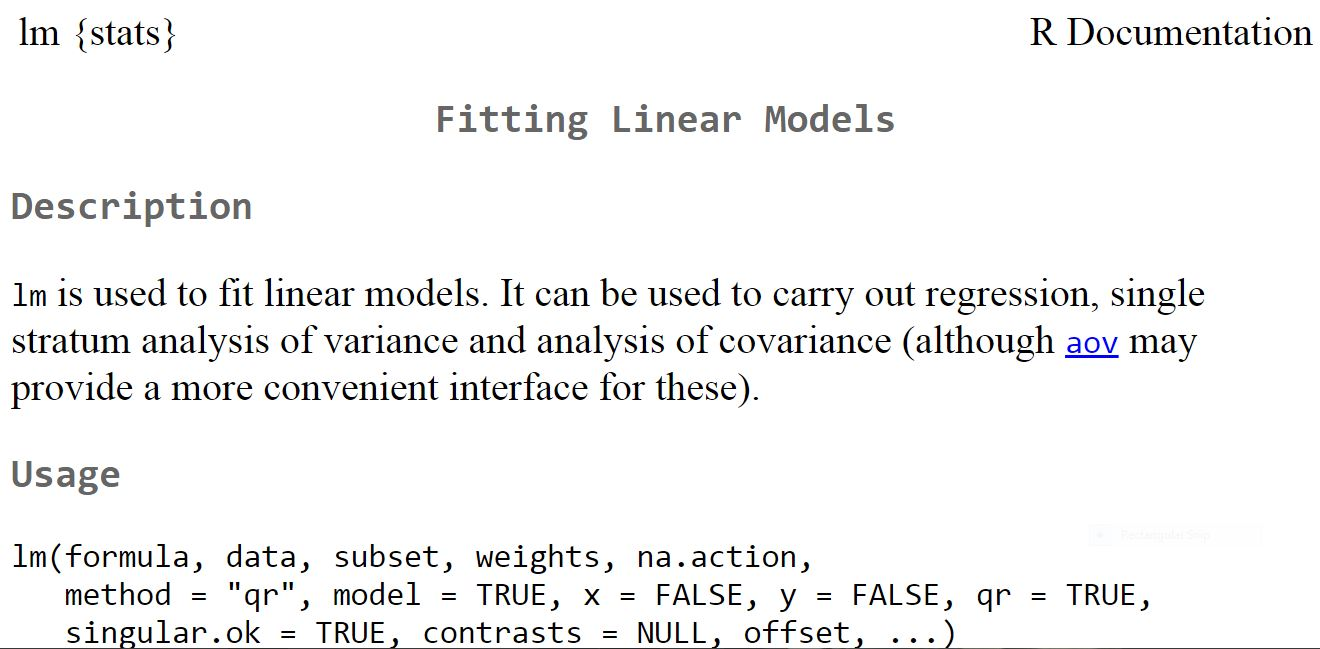
\includegraphics[width=1.1\linewidth]{images/LMhelpfile}
\end{figure}

\end{frame}
%=====================================================%
\begin{frame}[fragile]
\begin{framed}
	\begin{verbatim}
lm(formula, data, subset, weights, na.action,
method = "qr", model = TRUE, x = FALSE, y = FALSE, 
qr = TRUE, singular.ok = TRUE, contrasts = NULL, 
offset, ...)
	\end{verbatim}
\end{framed}

\textbf{ \texttt{weights}	} :\\ 
an optional vector of weights to be used in the fitting process. Should be NULL or a numeric vector. 
If non-NULL, weighted least squares is used with weights weights

\end{frame}
%=====================================================%
\begin{frame}
	\noindent \textbf{As an aside: Some useful Commands to know}
\Large


\begin{itemize}
\item \texttt{AIC} and \texttt{BIC}
\item \texttt{predict}
\item \texttt{confint}
\item \texttt{coef}
\item \texttt{influence}
\item dfbetas, dffits, covratio, cooks.distance
\end{itemize}
\end{frame}
%=====================================================%
\section{Residual Diagnostics}
\begin{frame}
	\LARGE
	\[\mbox{Regression Model Diagnostics }\]
\end{frame}
\begin{frame}
	\frametitle{John Fox - Companion to Applied Regression}
	\begin{figure}
\centering
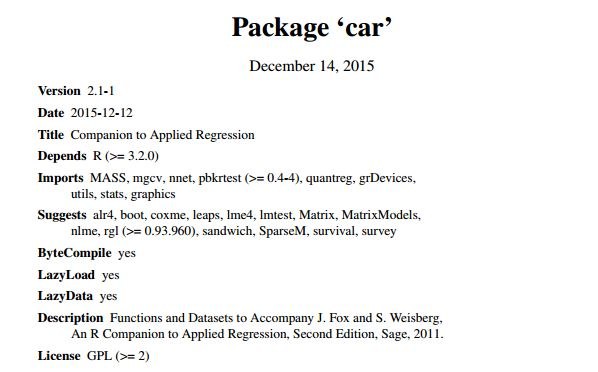
\includegraphics[width=1.1\linewidth]{images/CRAN-car}

\end{figure}

\end{frame}
%==========================================%
\begin{frame}[fragile]
	\frametitle{Residual Diagnostics - car package}
\large
\textbf{Outliers}
	\begin{framed}
		\begin{verbatim}
			# Assessing Outliers
		
		# Bonferonni p-value for most extreme obs
		outlierTest(fit) 
		
		#qq plot for studentized resid 
		qqPlot(fit, main="QQ Plot") 
		
		
		# leverage plots
		leveragePlots(fit) 
		
		\end{verbatim}
	\end{framed}
\end{frame}
%==========================================%
\begin{frame}[fragile]
	\frametitle{Residual Diagnostics}
	\large
	\begin{framed}
		\begin{verbatim}
		
		# Influential Observations
		# added variable plots 
		av.Plots(fit)
		
		# Cook's D plot
		# identify D values > 4/(n-k-1) 
		cutoff <- 4/((nrow(mtcars)-length(fit$coefficients)-2)) 
		plot(fit, which=4, cook.levels=cutoff)
		\end{verbatim}
	\end{framed}
\end{frame}
%==========================================%
\begin{frame}[fragile]
	\frametitle{Residual Diagnostics}
	\large
	\begin{framed}
		\begin{verbatim}		
		# Influence Plot 
		influencePlot(fit,	id.method="identify", 
		   main="Influence Plot")
		\end{verbatim}
	\end{framed}
\end{frame}
%==========================================%
\begin{frame}[fragile]
	\frametitle{Residual Diagnostics}
	\large
	\textbf{\textit{Non-constant Error Variance}}
	\begin{framed}
		\begin{verbatim}
		

		# Evaluate homoscedasticity
		# non-constant error variance test
		ncvTest(fit)
		
		# plot studentized residuals vs. fitted values 
		spreadLevelPlot(fit)
		\end{verbatim}
	\end{framed}
\end{frame}
%==========================================%
\begin{frame}[fragile]
	\frametitle{Residual Diagnostics}
	\large
	\noindent \textbf{Multi-collinearity}
	\begin{framed}
		\begin{verbatim}

		# Evaluate Collinearity
		
		vif(fit) # variance inflation factors 
		
		sqrt(vif(fit)) > 2 # problem?
		\end{verbatim}
	\end{framed}
\end{frame}
%==========================================%
\begin{frame}[fragile]
	\frametitle{Residual Diagnostics}
	\large
	\noindent \textbf{Nonlinearity}
	\begin{framed}
		\begin{verbatim}
		
		# Evaluate Nonlinearity
		# component + residual plot 
		crPlots(fit)
		
		# Ceres plots 
		ceresPlots(fit)
		\end{verbatim}
	\end{framed}
\end{frame}
%==========================================%
\begin{frame}[fragile]
	\frametitle{Residual Diagnostics}
	\large
	\textbf{Autocorrelation : Non-independence of Errors}
	\begin{framed}
		\begin{verbatim}
		
		
		# Test for Autocorrelated Errors
		durbinWatsonTest(fit)
		
		\end{verbatim}
	\end{framed}
\end{frame}
\begin{frame}
	\begin{figure}
\centering
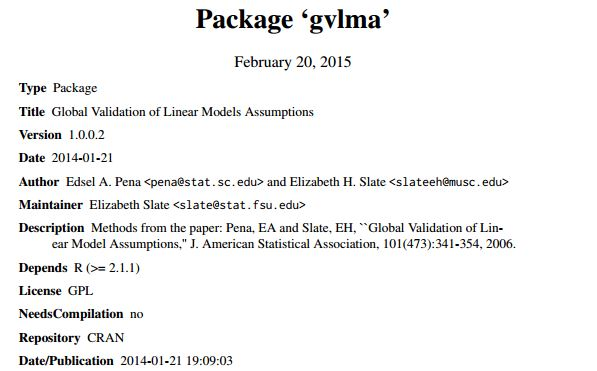
\includegraphics[width=1.1\linewidth]{images/CRAN-gvlma}
\caption{}
\label{fig:CRAN-gvlma}
\end{figure}

\end{frame}
%==========================================%
\begin{frame}[fragile]
	\frametitle{Residual Diagnostics}
	
	\noindent \textbf{Additional Diagnostic Help}\\
	The \texttt{gvlma( )} function in the gvlma package, performs a global validation of linear model assumptions as well separate evaluations of skewness, kurtosis, and heteroscedasticity.
	
	\begin{framed}
		\begin{verbatim}
		# Global test of model assumptions
		library(gvlma)
		gvmodel <- gvlma(fit) 
		summary(gvmodel)
		
		\end{verbatim}
	\end{framed}
\end{frame}
%==========================================%
\begin{frame}
	\frametitle{By The Way...}
	\Large
	\begin{itemize}
		\item 	The spellings homoskedasticity and heteroskedasticity are also frequently used.
		\item  J. Huston McCulloch argued that there should be a ``k" in the middle of the word and not a ``c".
		\item  His argument was that the word had been constructed in English directly from Greek roots rather than coming into the English language indirectly via the French. 
	\end{itemize}
	
	{
		\normalsize	
		\noindent \textit{See McCulloch, J. Huston (March 1985). "Miscellanea: On Heteros$\ast$edasticity". Econometrica 53 (2): 483. JSTOR 1911250.}
	}
\end{frame}
%=============================================== %

\section{Stepwise Regression}
\begin{frame}
	\LARGE
	\[\mbox{Stepwise  Regression}\]
\end{frame}
\begin{frame}
	\begin{figure}
		\centering
		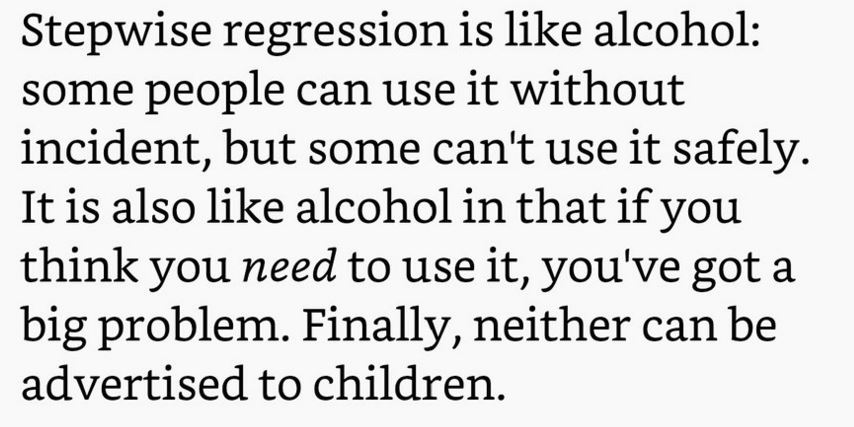
\includegraphics[width=1.1\linewidth]{images/StepwiseRegressionFischetti}
		\caption{Tony Fischetti}
		\label{fig:StepwiseRegressionFischetti}
	\end{figure}
	
\end{frame}
\begin{frame}
	\frametitle{Stepwise Regression}
	\large
	\begin{itemize}
		\item Stepwise regression is used when we deal with multiple independent variables. In this technique, the selection of independent variables is done with the help of an automatic process, which involves no human intervention.
		
		\item This feat is achieved by observing statistical values like R-square, t-stats and AIC metric to discern significant variables.
		\item Stepwise regression basically fits the regression model by adding/dropping predictor variables one at a time based on a specified criterion. 
		%Some of the most commonly used Stepwise regression methods are listed below:
		\item It is one of the method to handle higher dimensionality of data set.
		
	\end{itemize}
\end{frame}
%==============================================================================%
\begin{frame}
	\frametitle{Stepwise Regression}
	\Large
	\begin{itemize}
		\item \textbf{Standard stepwise regression} does two things. It adds and removes predictors as needed for each step.
		\item Forward selection starts with most significant predictor in the model and adds variable for each step.
		\item \textbf{Backward elimination} starts with all predictors in the model and removes the least significant variable for each step.
		\item The aim of this modeling technique is to maximize the prediction power with minimum number of predictor variables. \end{itemize}
	
\end{frame}
\begin{frame}[fragile]
\frametitle{Stepwise Regression}
\Large
\begin{framed}
	\begin{verbatim}
	#BACKWARD SELECTION
	FitBS = lm(mpg ~ . ,data=mtcars)
	step(FitAll, direction = "backward")
	
	#FORWARD SELECTION
	FitFS = lm(mpg ~ 1)
	step(FitAll, direction = "forward")
	\end{verbatim}
	\end{framed}
\end{frame}

\begin{frame}[fragile]
	\frametitle{Stepwise Regression}
	\Large
	\begin{framed}
		\begin{verbatim}
		library(MASS)
		fit <- lm(y~x1+x2+x3,data=mydata)
		stepwise <- stepAIC(fit, direction="both")
		
		stepwise$anova # display results
	\end{verbatim}
\end{framed}
\end{frame}
%==============================================================================%

\section{Polynomial Regression}
\begin{frame}
	\LARGE
	\[\mbox{Polynomial Regression}\]
\end{frame}

\begin{frame}
	\frametitle{Curvilinear Relationship}
	\begin{figure}
\centering
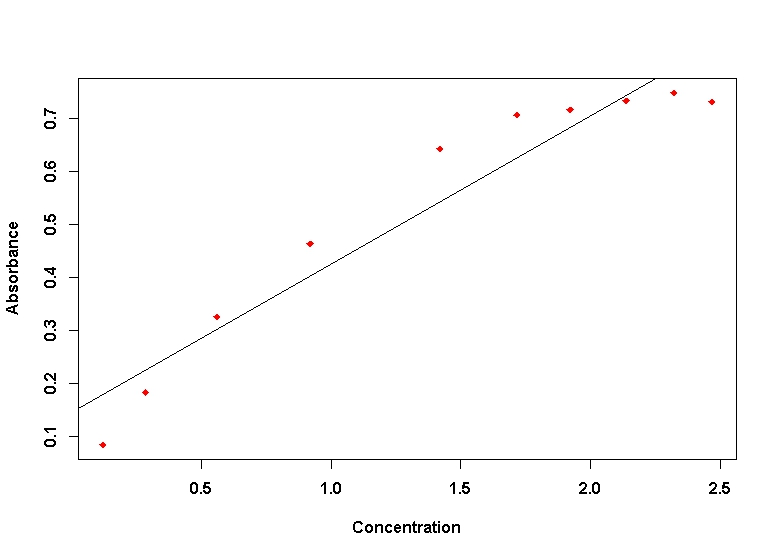
\includegraphics[width=1.0\linewidth]{images/ExamQ3plot}
\end{figure}

\end{frame}
\begin{frame}
\frametitle{Specifying Polynomial Models}
	\begin{figure}
\centering
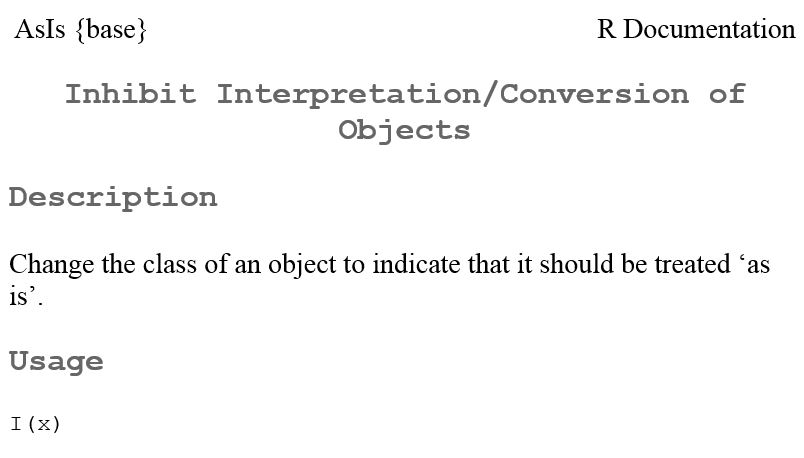
\includegraphics[width=1.0\linewidth]{images/I-Functions}

\end{figure}

\end{frame}
%==============================================================================%
\begin{frame}
	\noindent \textbf{Polynomial Regression}
\large	
	\begin{itemize}
\item Suppose that, when you inspect the data, the best fit line is not a straight line, rather a curve that fits into the data points.
\item 	A regression equation is a polynomial regression equation if the power of independent variable is more than 1. 
\item The equation below represents a quadratic equation:
	
	\[	y=b_0+ +b_1x + b_2x^2\]


	\end{itemize}
\end{frame}
%==============================================================================%
\begin{frame}
	\noindent \textbf{Polynomial Regression}	
	\large
\begin{figure}
\centering
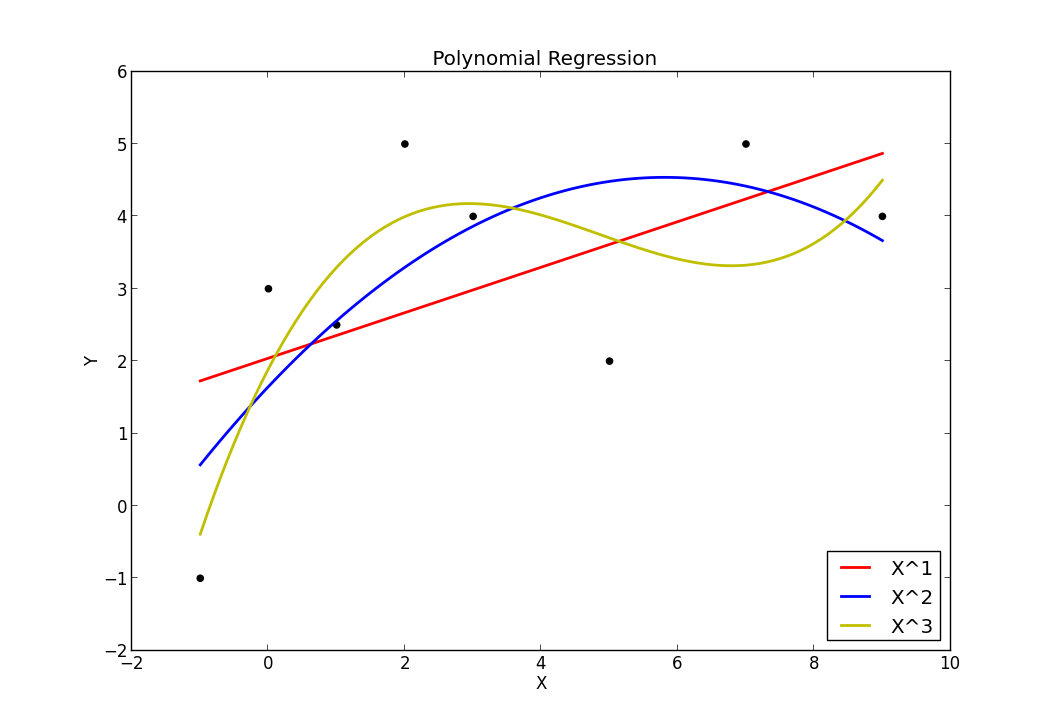
\includegraphics[width=1.1\linewidth]{images/polynomial1}

\end{figure}

	
	
\end{frame}
%=============================================================%
\begin{frame}
		\noindent \textbf{Polynomial Regression}	
		\large
\begin{figure}
\centering
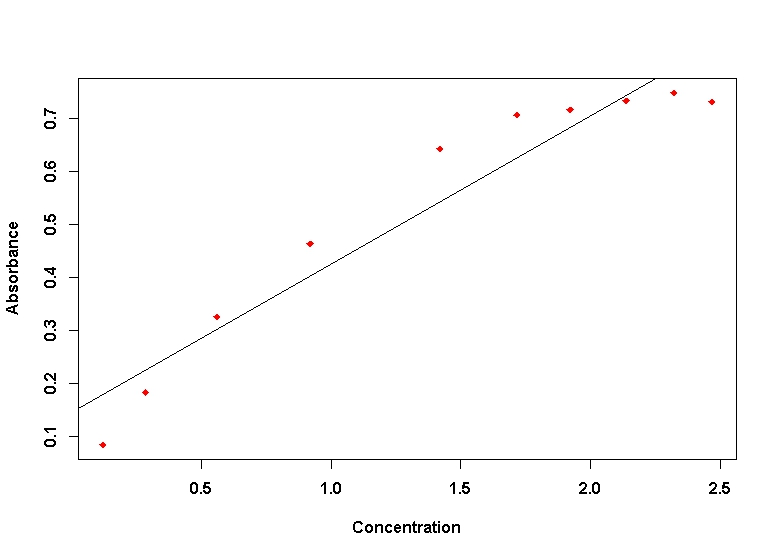
\includegraphics[width=1.1\linewidth]{images/ExamQ3plot}
\caption{}
\label{fig:ExamQ3plot}
\end{figure}

\end{frame}
\begin{frame}[fragile]
	\large
	\begin{framed}
	\begin{verbatim}
	# Absorbance 
	x<-c(0.084, 0.183, 0.326, 0.464, 0.643, 
	0.707, 0.717, 0.734, 0.749, 0.732)
	
	# Concentration 
	y<-c(0.123, 0.288, 0.562, 0.921, 1.420, 
	1.717, 1.921, 2.137, 2.321, 2.467)
	
	\end{verbatim}
	\end{framed}
	\begin{itemize}
		\item Compare linear, quadratic and cubic fit.
	\end{itemize}
\end{frame}
%========================================================= %
\begin{frame}[fragile]
\frametitle{Polynomial Regression}
		\Large
		Fitting a polynomial of degree 3.
	\begin{framed}
		\begin{verbatim}
		lm(y ~ x + I(x^2) + I(x^3))
	
		
		lm(y ~ poly(x, 3))
		\end{verbatim}
	\end{framed}
\end{frame}
%==============================================================================%
\begin{frame}
	\frametitle{Polynomial Regression}
\textbf{Important Points:}
	
	\begin{itemize}
\item 	While there might be a temptation to fit a higher degree polynomial to get lower error, this can result in \textbf{over-fitting}. \item Always plot the relationships to see the fit and focus on making sure that the curve fits the nature of the problem. 
\item Here is an example of how plotting can help:
	underfitting-overfitting
	
\item 	Especially look out for curve towards the ends and see whether those shapes and trends make sense. Higher polynomials can end up producing weird results on extrapolation.
	\end{itemize}

	
\end{frame} 
%======================================================== %

\section{Segmented Regression}
\begin{frame}
	\LARGE
	\[\mbox{Segmented Regression}\]
\end{frame}
%=====================%
\begin{frame}
		\frametitle{Segmented Regression}
		\large
	\begin{figure}
\centering
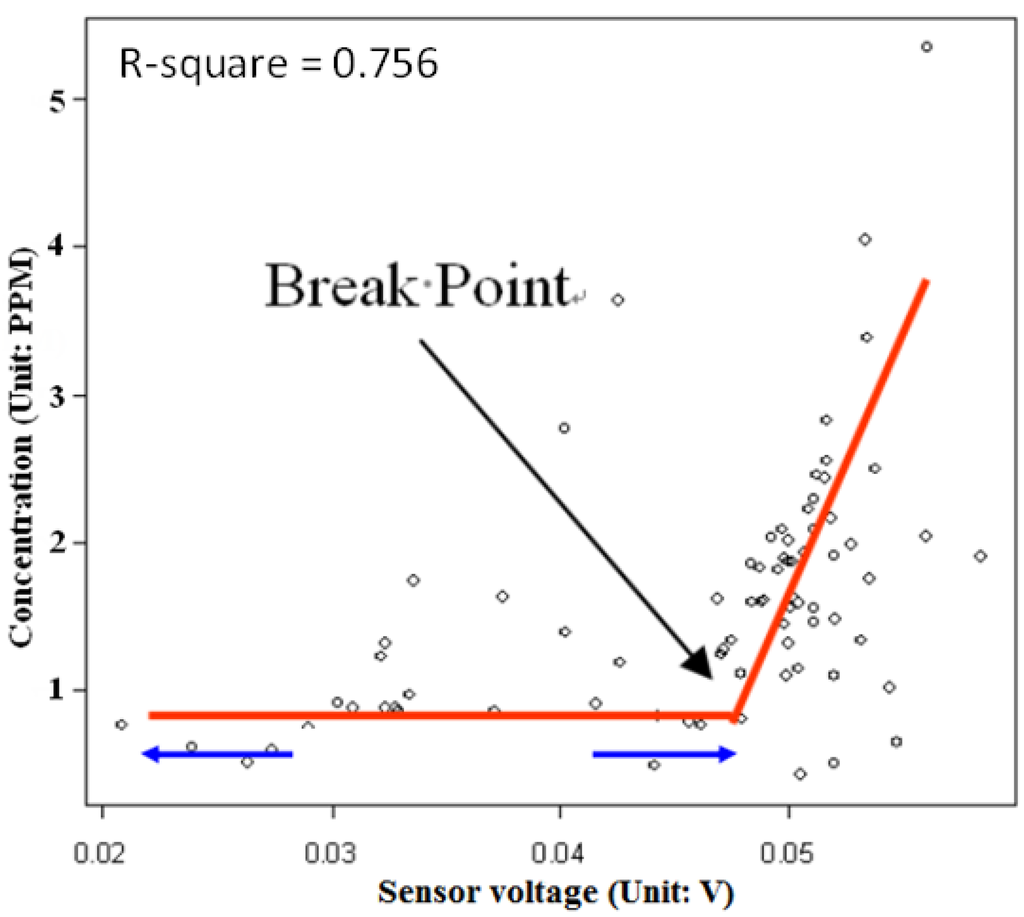
\includegraphics[width=0.7\linewidth]{images/breakpoint}
\caption{}
\label{fig:breakpoint}
\end{figure}

\end{frame}

%======================================================= %
%%- https://rpubs.com/MarkusLoew/12164

%%- http://stats.stackexchange.com/questions/20890/how-to-use-segmented-package-to-fit-a-piecewise-linear-regression-with-one-break
\begin{frame}
			\frametitle{Segmented Regression}
			\large
			\begin{itemize}
		\item	\textbf{Segmented regression} is a method in regression analysis in which the independent variable is partitioned into intervals and a separate line segment is fit to each interval. 
			
		\item	Segmented regression analysis can also be performed on multivariate data by partitioning the various independent variables. \item Segmented regression is useful when the independent variables, clustered into different groups, exhibit different relationships between the variables in these regions. 
		\item The boundaries between the segments are \textbf{breakpoints}.
%			
%		\item	Segmented linear regression is segmented regression whereby the relations in the intervals are obtained by linear regression.
			\end{itemize}

\end{frame}
%======================================================= %
\begin{frame}
		\frametitle{Segmented Regression}
		\large
	\begin{figure}
\centering
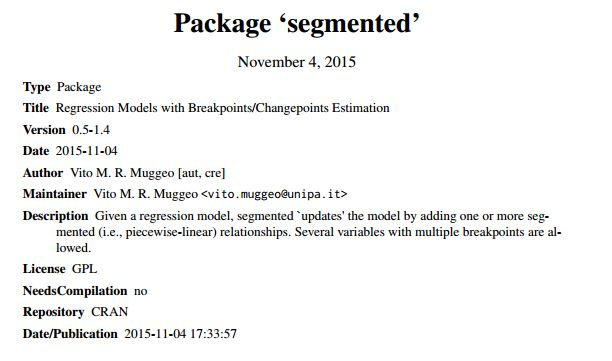
\includegraphics[width=1.1\linewidth]{images/CRAN-segmented}


\end{figure}

\end{frame}


\begin{frame}
	\frametitle{Segmented Regression}
	\large
	
	\begin{figure}
\centering
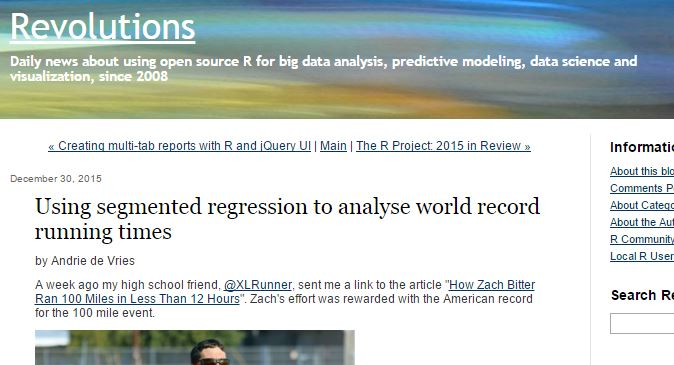
\includegraphics[width=1.1\linewidth]{images/Segmented1}
\end{figure}
\end{frame}
%============================================================= %
\begin{frame}
	\frametitle{Segmented Regression}
	\large
	
	\begin{figure}
		\centering
		\includegraphics[width=1.1\linewidth]{images/Segmented2}

	\end{figure}
	
\end{frame}

%============================================================= %
\begin{frame}
	\frametitle{Segmented Regression}
\large
\begin{itemize}
\item The \texttt{segmented()} function allows you to modify a fitted object of class \texttt{lm} or \texttt{glm}, specifying which of the independent variables should have segments (kinks).  

\item In my case, I fitted a linear model with a single variable (log of distance), and allowed \texttt{segmented()} to find a single kink point.
\end{itemize}

\end{frame}

\begin{frame}
	\frametitle{Segmented Regression}
	\large
\begin{itemize}
\item First fit a generic linear model, then use the \texttt{segmented()} function to fit the piecewise regression.
\item  The \texttt{segmented()} function takes for its arguments the generic linear model, \texttt{seg.Z} which is a one sided formula describing the predictor with a segment 
\item \texttt{psi} is a starting value of the breakpoint. 
\end{itemize}
\end{frame}
\begin{frame}[fragile]
\frametitle{Segmented Regression}
\large
\begin{framed}
	\begin{verbatim}
#Andrie De Vries's Model

# Fit linear model
lfit <- lm(Speed ~ logDistance, data = modeldata)

# Fit segmented model
sfit <- segmented(lfit, seg.Z = ~ logDistance)

#Identify Breakpoints
exp10(sfit$psi)
summary(sfit)
	
	\end{verbatim}
	\end{framed}
\end{frame}

%======================================================= %

\section{Weighted Regression}
\begin{frame}
	\LARGE
	\[\mbox{Weighted Regression}\]
\end{frame}
\begin{frame}
	\frametitle{Heteroskedascity}
	\large
	\begin{figure}
		\centering
		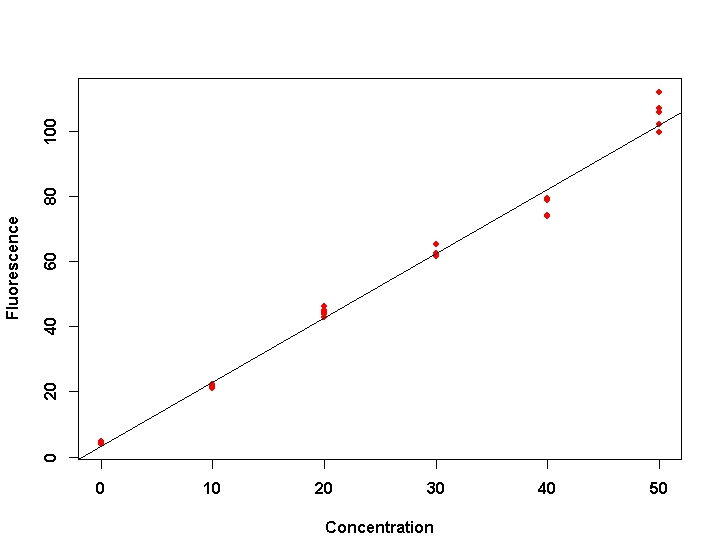
\includegraphics[width=1.0\linewidth]{images/ExamQ2plot2}
	\end{figure}
	
\end{frame}

%=============================================== %
\begin{frame}
	\frametitle{Heteroskedascity}
	\large
	\begin{figure}
		\centering
		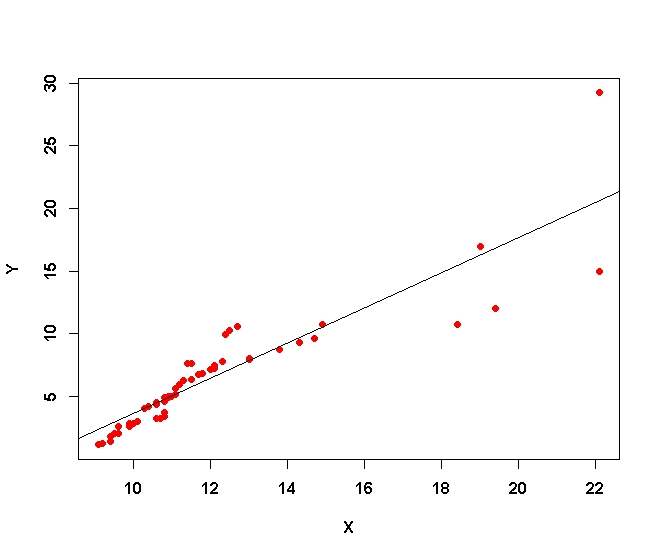
\includegraphics[width=0.95\linewidth]{images/ExamQ2plot}
	\end{figure}
	
\end{frame}
%=============================================== %
\section{Robust Regression}
\begin{frame}
	\LARGE
	\[\mbox{Robust Regression}\]
\end{frame}
\begin{frame}
	\frametitle{Robust Regression}
	\large
\begin{itemize}
	\item When fitting a least squares regression, we might find some outliers or high leverage data points.
	\item However data points are not data entry errors, neither they are from a different 
	population than most of our data. 
	\item No proper reason to exclude them from the analysis. 
\end{itemize}
\end{frame}

%==============================================================================%

\begin{frame}
	\frametitle{Robust Regression}
	\large
\begin{itemize}
	\item Robust regression might be a good strategy since it is a compromise between excluding these points 
	entirely from the analysis and including all the data points and treating all them equally in OLS 
	regression. 
	\item 
	The idea of robust regression is to weigh the observations differently based on how well 
	behaved these observations are. 
\end{itemize}
\end{frame}
\begin{frame}
	\frametitle{Robust Regression}
	\begin{itemize}
		\item When fitting a least squares regression, we might find some outliers or high leverage data points. 
		\item We have decided that these data points are not data entry errors, neither they are from a different 
		population than most of our data. So we have no proper reason to exclude them from the analysis. 
	\end{itemize}
\end{frame}
%===================================== %
\begin{frame}
	\frametitle{Robust Regression}
	\begin{itemize}
		\item Robust regression might be a good strategy since it is a compromise between excluding these points 
		entirely from the analysis and including all the data points and treating all them equally in OLS 
		regression. 
		\item The idea of robust regression is to weigh the observations differently based on how well 
		behaved these observations are.
	\end{itemize}
	
\end{frame}
%===================================== %
\begin{frame}
	\frametitle{Robust Regression}
	\large
	There are several weighting functions that can be used for Robust Regression. 
	
	\begin{itemize}
		\item Huber
		\item Hampel
		\item Bisquare
	\end{itemize}
	\end{frame}
	\begin{frame}
		\frametitle{Robust Regression}
		\large
		\noindent \textbf{Huber Weighting}\\
		In Huber weighting, observations with small residuals get a weight of 1 and the larger the residual, the smaller the weight. 
		
		\bigskip
		
		This is defined by the weight function \begin{equation} w(e) = \left\{ \begin{array}{rl} 1 &\mbox{for $|e| <= k$} \\ \frac{k}{|e|} &\mbox{for $|e| > k$} \end{array} \right. \end{equation}
	\end{frame}
	
	\begin{frame}

				\frametitle{Robust Regression}
				\large
				\noindent \textbf{Tuning Constant}
		\begin{itemize}		
\item 	The value k for the Huber and bisquare estimators is called a \textbf{tuning constant}
\item Smaller values of k produce
	more resistance to outliers, but at the expense of lower efficiency when the errors are normally distributed.
\item 	The tuning constant is generally picked to give reasonably high efficiency in the normal case; in particular,
	$k = 1.345\sigma$ for the Huber and $k = 4.685\sigma$ for the bisquare (where $\sigma$ is the standard deviation of the errors)
	produce 95-percent efficiency when the errors are normal, and still offer protection against outliers.
		\end{itemize}
	
	\end{frame}
\begin{frame}
	\frametitle{Robust Regression}
	\large
	\begin{itemize}
	\item The idea of robust regression is to weigh the observations differently based on how well behaved 
	these observations are. 
	\item Roughly speaking, it is a form of weighted and reweighted least squares 
	regression (i.e. a two step process , first fitting a linear model, then a robust model to correct for the 
	influence of outliers). 
	\item 
	Robust regression is done by\textbf{ iterated re-weighted least squares (IRLS)}.
	\item  The rlm command in the 
	MASS package command implements several versions of robust regression. 
	\end{itemize}
\end{frame}

\begin{frame}
	\frametitle{Median Based Linear Models}
	\begin{figure}
\centering
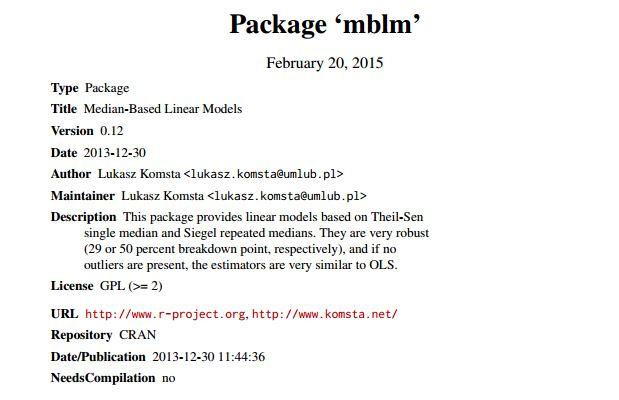
\includegraphics[width=1.1\linewidth]{images/theilRegression}
\caption{}
\label{fig:theilRegression}
\end{figure}

\end{frame}
%==============================================================================%
\section{Censored Regression}
\begin{frame}
	\LARGE
	\[\mbox{Censored Regression}\]
\end{frame}
%------------------- %
%\begin{frame}
%	\frametitle{Censored Regression}
%	\begin{itemize}
%\item	Censored regression models commonly arise in cases where the variable of interest is only observable under certain conditions. 
%\item A common example is labor supply. Data are frequently available on the hours worked by employees, and a labor supply model estimates the relationship between hours worked and characteristics of employees such as age, education and family status. 
%	\end{itemize}
%
%\end{frame}
%==============================================================================%
%\begin{frame}
%	\frametitle{Censored Regression}	
%	However, such estimates undertaken using linear regression will be biased by the fact that for people who are unemployed it is not possible to observe the number of hours they would have worked had they had employment. Still we know age, education and family status for those observations.
%	
%	A model commonly used to deal with censored data is the Tobit model, including variations such as the Tobit Type II, Type III, and Type IV models.
%\end{frame}

\begin{frame}
	\frametitle{Censored Models: Tobit Regression}
	\large
	\textbf{Examples of Tobit Analysis}\\
	In the 1980s there was a federal law restricting speedometer readings to no more than 85 mph. So if you wanted to try and predict a vehicle's top-speed from a combination of horse-power and engine size, you would get a reading no higher than 85, regardless of how fast the vehicle was really traveling. 
	
	This is a classic case of right-censoring (censoring from above) of the data. The only thing we are certain of is that those vehicles were traveling at least 85 mph.
\end{frame}
%======================================================================== %
\begin{frame}
	\frametitle{Censored Models: Tobit Regression}
	\large
	\textbf{Examples of Tobit Analysis}
	\begin{itemize}
\item 	A research project is studying the level of lead in home drinking water as a function of the age of a house and family income. 
\item The water testing kit cannot detect lead concentrations below 5 parts per billion (ppb). 
\item	
	The EPA considers levels above 15 ppb to be dangerous. These data are an example of left-censoring (censoring from below).
	\end{itemize}

\end{frame}
%======================================================================== %
\begin{frame}[fragile]
		\frametitle{Censored Models: Tobit Regression}
		\large
		\textbf{Examples of Tobit Analysis}\\
		\begin{itemize}

\item Consider the situation in which we have a measure of academic aptitude (scaled 200-800) which we want to model using reading and math test scores, as well as, the type of program the student is enrolled in (academic, general, or vocational). 
\item The problem here is that students who answer all questions on the academic aptitude test correctly receive a score of 800, even though it is likely that these students are not "truly" equal in aptitude. 
\item The same is true of students who answer all of the questions incorrectly. All such students would have a score of 200, although they may not all be of equal aptitude.
		\end{itemize}
	
\end{frame}
\begin{frame}
	\frametitle{Censored Models: Tobit Regression}
	\textbf{Tobit Regression}\\
	The tobit model, also called a censored regression model, is designed to estimate linear relationships between 
	variables when there is either left- or right-censoring in the dependent variable (also known as censoring from below and 
	above, respectively). 
\end{frame}
%===============================================================================================================================%
\begin{frame}
	\frametitle{Censored Models: Tobit Regression}
	\textbf{Censoring}\\
	Censoring from above takes place when cases with a value at or above some threshold, all take on the value of 
	that threshold, so that the true value might be equal to the threshold, but it might also be higher. 
	In the case of censoring from below, values those that fall at or below some threshold are censored.
\end{frame}
%===============================================================================================================================%
\begin{frame}
	\begin{figure}
		\centering
		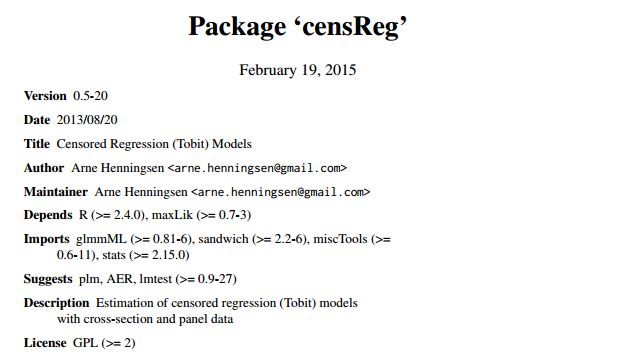
\includegraphics[width=1.1\linewidth]{images/CRAN-censreg}
		
	\end{figure}
	
\end{frame}
%=============================================================%
%======================================================================== %
\begin{frame}[fragile]
\frametitle{Censored Models: Tobit regression}
\large
We run the tobit model, using the \texttt{vglm()} function of the \textbf{VGAM} package.
	\begin{figure}
\centering
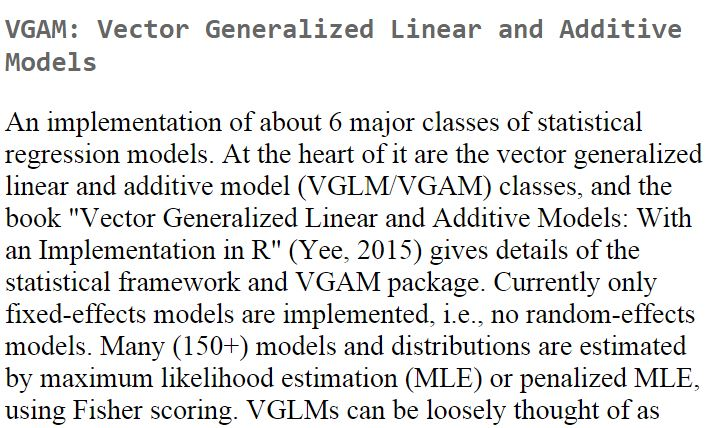
\includegraphics[width=0.7\linewidth]{images/cran-Vgam}
\end{figure}

\end{frame}

%================================= %
\begin{frame}[fragile]
	\large
	\begin{verbatim}
	library(VGAM)
	summary(m <- vglm(apt ~ read + math + prog, 
	             tobit(Upper = 800), data = dat))


	## Call:
	## vglm(formula = apt ~ read + math + prog, family = tobit(Upper = 800), 
	##     data = dat)
	## 
	## Pearson Residuals:
	##          Min    1Q Median   3Q Max
	## mu      -2.6 -0.76 -0.051 0.79 4.1
	## log(sd) -1.1 -0.62 -0.369 0.25 5.4
\end{verbatim}
\end{frame}
%================================= %
\begin{frame}[fragile]
	\large
\begin{verbatim}
	## Coefficients:
	##                Estimate Std. Error z value
	## (Intercept):1     209.6     32.457     6.5
	## (Intercept):2       4.2      0.053    79.4
	## read                2.7      0.618     4.4
	## math                5.9      0.705     8.4
	## proggeneral       -12.7     12.355    -1.0
	## progvocational    -46.1     13.770    -3.4
\end{verbatim}
\end{frame}
%================================= %
\begin{frame}[fragile]
	\large
	\begin{verbatim}
	## Number of linear predictors:  2 
	## 
	## Names of linear predictors: mu, log(sd)
	## 
	## Dispersion Parameter for tobit family:   1
	## 
	## Log-likelihood: -1041 on 394 degrees of freedom
	## 
	## Number of iterations: 4
\end{verbatim}
\end{frame}

\section{Truncated Regression}
\begin{frame}
	\LARGE
	\[\mbox{Truncated Regression}\]
\end{frame}
\begin{frame}[fragile]
	\frametitle{Truncated and Censored Regression}
	\large
	\begin{itemize}
		\item Censored regression models are often confused with truncated regression models. 
		\item Truncated regression models are used for data where whole observations are missing so that the values for the dependent and the independent variables are unknown. \item Censored regression models are used for data where only the value for the dependent variable  is unknown while the values of the independent variables are still available.
	\end{itemize}
	
\end{frame}
%======================================== %
\begin{frame}
	\frametitle{Truncated Regression}
	\noindent \textbf{Case Studies 1}
	\begin{itemize}
		\item One example of truncated samples come from historical military height records. Many armies imposed a minimum height requirement on soldiers. 
		\item This implies that men shorter than the MHR are not included in the sample. 
		\item This implies that samples drawn from such records are statistically incomplete, in as much as a substantial portion of the underlying population's height distribution is unavailable for analysis. 
		\item Consequently, without proper statistical correction, any results obtained from such deficient samples, such as means, correlations, or regression coefficients are wrong (biased). 
	\end{itemize}
\end{frame}
\begin{frame}
	\frametitle{Truncated Regression}
	\noindent \textbf{Case Studies 2}
	\begin{itemize}
		\item A study of students in a special GATE (gifted and talented education) program wishes to model achievement as a function of language skills and the type of program in which the student is currently enrolled. 
		\item A major concern is that students are required to have a minimum achievement score of 40 to enter the special program. 
		\item Thus, the sample is truncated at an achievement score of 40.
		\end{itemize}
	\end{frame}	
%==================================%

\begin{frame}
	\frametitle{Truncated Regression}
	\large
	\begin{itemize}
		\item 
		In such a case truncated regression has the considerable advantage of immediately providing consistent and unbiased estimates of the coefficients of the independent variables, as well as their standard errors, thereby allowing for further statistical inference, such as the calculation of the t-values of the estimates.
	\end{itemize}
\end{frame}
\begin{frame}
	\frametitle{Truncated Regression}
	\large
	\begin{figure}
		\centering
		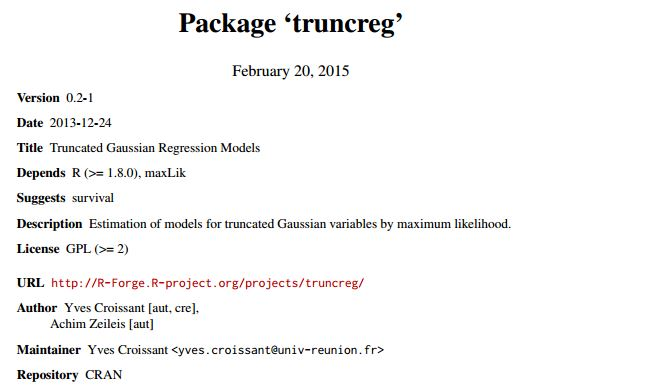
\includegraphics[width=1.1\linewidth]{images/CRAN-truncreg}
		\caption{}
		\label{fig:CRAN-truncreg}
	\end{figure}
	
\end{frame}
\begin{frame}[fragile]
\frametitle{Truncated regression}
\large
\begin{itemize}
\item Use the \texttt{truncreg} function in the \textbf{truncreg} package to estimate a truncated regression model. 
\item The \texttt{point} argument indicates where the data are truncated, and the direction indicates whether it is left or right truncated.

\end{itemize}

\begin{framed}
\begin{verbatim}
m <- truncreg(achiv ~ langscore + prog, 
   data = dat, point = 40, direction = "left")
\end{verbatim}
\end{framed}

\end{frame}
\section{Deming Regression}
\begin{frame}
	\LARGE
	\[\mbox{Deming Regression}\]
\end{frame}
\begin{frame}
	\frametitle{Deming Regression}
	\begin{figure}
		\centering
		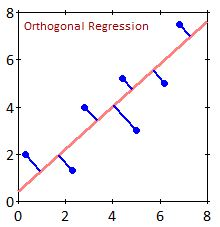
\includegraphics[width=0.35\linewidth]{images/OrthogonalRegression}
		
		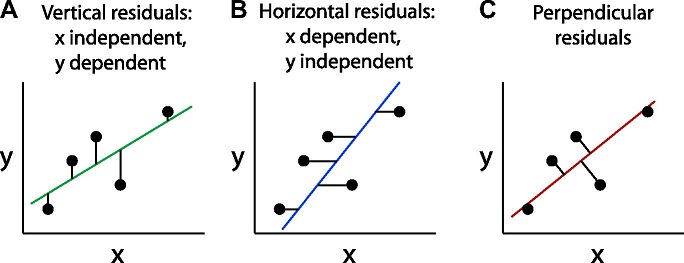
\includegraphics[width=0.8\linewidth]{images/elife_regressions}
		
	\end{figure}
	
\end{frame}
\begin{frame}
	\frametitle{Deming Regression}
	\large
	\begin{itemize}
		\item	An ion-selective electrode (ISE) determination of sulphide from sulphate-reducing bacteria was compared with a gravimetric determination. 
		\item Each pair of determinations were taken from the same sample. 
		\item The results obtained by both methods are expressed in milligrams of sulphide, and are tabulated below.
	\end{itemize}
	
	\begin{center}
		\begin{tabular}{|c|ccccccc|}
			\hline
			% after \\: \hline or \cline{col1-col2} \cline{col3-col4} ...
			ISE method & 108 & 102& 152 & 73 & 106 & 114 &  128   \\
			gravimetry & 105 & 96& 113 & 91 & 108 &  101 & 141  \\ 
			\hline
			\hline
			% after \\: \hline or \cline{col1-col2} \cline{col3-col4} ...
			ISE method & 85 & 106 & 114 &  128 & 142& 160& 128 \\
			gravimetry &  91 & 108 &  101 & 141 & 161 & 182& 118\\
			\hline
		\end{tabular}
	\end{center}
	
\end{frame}
%===================================================== %
\begin{frame}
	\frametitle{Deming Regression}	\begin{figure}
		\centering
		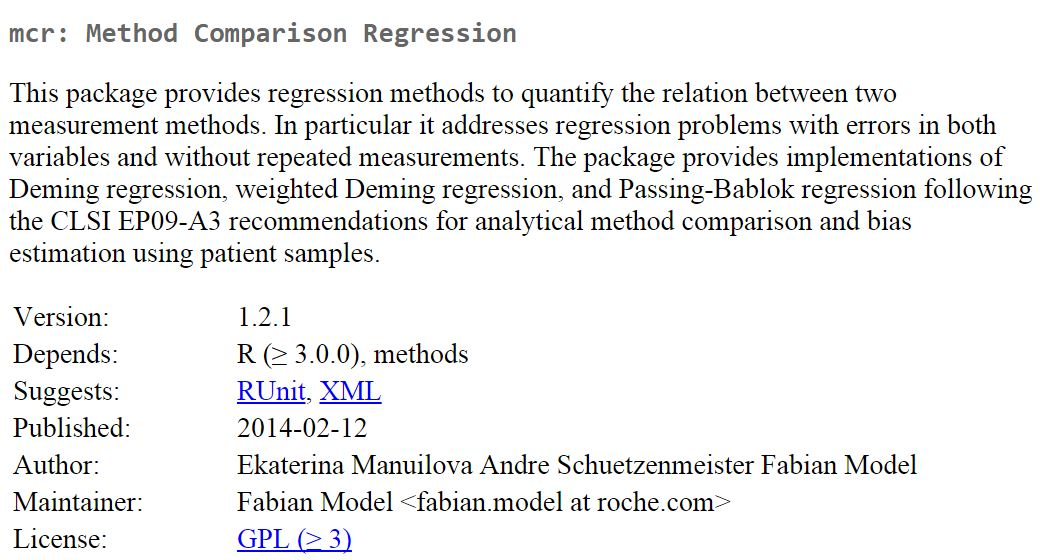
\includegraphics[width=1.1\linewidth]{images/CRAN-mcr}
		
	\end{figure}
	
\end{frame}
%===================================================== %
\begin{frame}
	\frametitle{Deming Regression}
	\begin{figure}
		\centering
		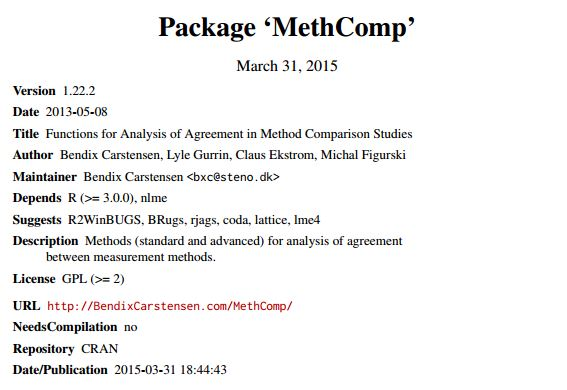
\includegraphics[width=1.1\linewidth]{images/CRAN-MethComp}
		
	\end{figure}
	
\end{frame}
%==============================================================================%
\end{document}
